\documentclass[preprint,12pt]{elsarticle}

\usepackage[T1]{fontenc}
\usepackage{lmodern}
\usepackage{amsmath,amssymb,amsfonts,amsthm}
\usepackage{algorithmic}
\usepackage{algorithm}
\usepackage{graphicx}
\usepackage{textcomp}
\usepackage{xcolor}
\usepackage{tikz}
\usepackage{pgfplots}
\usepackage{pgfplotstable}
\usepackage{booktabs}
\usepackage{multirow}
\usepackage{xurl}
\usepackage[colorlinks=true, urlcolor=blue, linkcolor=blue, citecolor=blue]{hyperref}
\usepackage{balance}
\usepackage{array}
\usepackage{soul}
\sethlcolor{yellow}
\usepackage{tcolorbox}
\tcbuselibrary{skins,breakable}
\newtcolorbox{hlblock}{
	colback=yellow!45,
	colframe=yellow!85!orange,
	arc=2pt,
	boxrule=0.8pt,
	left=4pt,right=4pt,top=4pt,bottom=4pt,
	breakable
}
\newcommand{\hlcrit}[1]{\textcolor{red}{\textbf{#1}}}

\usetikzlibrary{shapes.geometric,arrows.meta,positioning,fit,backgrounds,calc,patterns}
\pgfplotsset{compat=1.18}
\interfootnotelinepenalty=10000

\newtheorem{definition}{Definition}
\newtheorem{remark}{Remark}

\definecolor{tcblue}{RGB}{31,97,171}
\definecolor{tcgreen}{RGB}{39,139,60}
\definecolor{tcorange}{RGB}{196,98,16}
\definecolor{tcgray}{RGB}{100,100,110}
\definecolor{tcred}{RGB}{170,30,30}
\definecolor{tcpurple}{RGB}{110,40,160}
\definecolor{tclightblue}{RGB}{214,234,255}
\definecolor{tclightgreen}{RGB}{209,244,214}
\definecolor{tclightorange}{RGB}{253,226,198}
\definecolor{tclightgray}{RGB}{238,238,242}

\hyphenation{TrajectoryCache}

\begin{document}
	
	\begin{frontmatter}
		
		\title{TrajectoryCache: Benchmarking Rule-Based versus Online Reinforcement Learning Edge Caching Under Vehicular Mobility and Positioning Uncertainty}
		
		\author[1]{Adeel Ahmad\corref{cor1}}
		\ead{443057803@stu.iu.edu.sa}
		
		\author[1,2]{Ali Akrma}
		
		\author[1]{Touqeer Ali Syed}
		
		\cortext[cor1]{Corresponding author}
		
		\address[1]{AI Center, Faculty of Computer and Information Systems, Islamic University of Madinah, Madinah 42351, Saudi Arabia}
		
		\address[2]{AI V\&V Lab, King Fahd University of Petroleum and Minerals, Dhahran, Saudi Arabia}
		
	
		\begin{abstract}
		Location-specific content delivery in vehicular edge computing faces non-stationary demand driven by high vehicle mobility and dynamic traffic density. Existing caching literature typically evaluates either single heuristic algorithms or complex reinforcement learning schemes against classical temporal baselines, rarely comparing rule-based heuristics directly against learning-based policies under identical multi-seed protocols and physical positioning uncertainty. In this paper, we present a systematic comparative benchmark study evaluating six distinct cache replacement paradigms: classical temporal frequency/recency policies (LRU, LFU, FIFO, Random), a pure spatial proximity heuristic (ProximityCache), a spatial-urgency-augmented rule-based policy (TrajectoryCache), and a learning-based Temporal-Difference Q-Learning policy (QLearningCache). Evaluated across a 10 km highway simulation across 10 independent random seeds under rigorous non-overlapping evaluation windows, we report three core comparative insights. First, rule-based spatial-popularity augmentation achieves the lowest mean miss rate ($52.05 \pm 1.35$\% at Zipf $\alpha=0.8$), outperforming both classical LFU ($52.85 \pm 1.58$\%, Wilcoxon $p=0.042$) and tabular Q-Learning ($53.42 \pm 1.48$\%). Second, a density sensitivity sweep establishes an empirical crossover boundary: rule-based spatial urgency provides significant gains under sparse and moderate vehicular density ($n \leq 200$) by anticipating localized demand bursts, whereas learning-based and classical LFU policies converge at saturated urban density ($n \geq 400$). Third, sensitivity analysis under GNSS positioning noise ($0$--$15$ meters) and update latency ($0$--$3$ seconds) reveals that while rule-based policies degrade gracefully under telemetry error, learning-based policies exhibit higher variance during online value adaptation. Finally, wall-clock computational profiling demonstrates that closed-form rule-based scoring executes in sub-millisecond per-decision time, whereas online TD learning incurs orders of magnitude higher training overhead, clarifying the practical trade-offs between heuristic simplicity and learning flexibility.
		\end{abstract}
		
		\begin{keyword}
			Vehicular edge caching \sep cache replacement \sep spatial urgency \sep content popularity \sep vehicle platooning \sep time-to-encounter \sep miss rate \sep MEC
		\end{keyword}
		
	\end{frontmatter}
	
	\section{Introduction}

	\label{sec:intro}
	
	Connected and autonomous vehicles create huge demand for dynamic, location-specific content. Low latency is crucial for high-definition map tile streaming, real-time traffic updates, dashboard overlays with AR, and localized point-of-interest data \cite{zhang2020mobile}. Serving this volume from centralized cloud data centers introduces round-trip propagation delays and congestion in the mobile core. This has led to a wide proliferation of Multi-access Edge Computing (MEC) applications, which place storage and compute at the network edge, often co-located with Roadside Units (RSUs) or cellular base stations, near the road traffic \cite{taleb2017multi, Cao_2020, Yousefpour_2019, Khan_2019}. Edge-deployed caches meet latency-critical requests within the local network, reducing response times and relieving the backhaul \cite{pham2020survey, bastug2014living}.
	
	In a vehicular network, however, there is a challenge that is very different from fixed-access networks: extreme spatial and temporal variability of the client pool. At highway speeds, a single car can travel an RSU's coverage area in tens of seconds. The population around a specific cache is thus constantly changing. Classical replacement policies make the assumption of a relatively stable client population. LRU stores content based on the absolute timing of past access to that content only, and has no predictive capabilities for approaching vehicles. Under consistent usage, LFU is efficient, but it cannot deal with short-time bursts of usage in a locality before they die out. 
	
	This is especially apparent when distinct traffic clusters pass through the coverage area of the cache. On highways, typical car-following behaviors generate clusters of closely spaced cars that arrive together. When such a cluster enters the coverage area, it creates a burst of requests for geographically close content. The frequency statistics collected during quieter times give false indications of the instantaneous demand profile. A cache strictly managed by LFU retains items favored by the long-run popularity distribution rather than the specific items that the physically present vehicles are currently seeking. 
	
	We propose \textbf{TrajectoryCache} (TC), a lightweight cache replacement heuristic that caters to both past popularity and current physical need. TC extends frequency-based caching by adding a spatial urgency signal that is calculated from the relative positions, speeds, and headings of nearby vehicles relative to the locations of the cached content items. Popularity is a strong statistical anchor supported by TC's closed-form urgency term, thereby ensuring that content is kept in the cache that is both historically popular and physically imminent. This enables the edge cache to anticipate the localized demand spikes that pure frequency tracking would not be able to capture until it is too late. 
	
	The operational setting involves an edge cache located on a highway, with a continuous stream of passing vehicles. Each content item in the catalog has a physical location along the road (for example, an intersection's HD map tile). Vehicles actively request items located ahead of them within a certain relevance range. The edge cache has limited capacity, so it needs to continually make decisions about what to retain, executing a replacement decision each time it receives a cache miss when the cache is full.
	
	\textbf{Contributions.} We make the following contributions:
	\begin{itemize}
		\item We present a heuristic that aggregates normalized spatial urgency (based on linear time-to-encounter estimates of nearby vehicles) and normalized content popularity (based on the number of requests received in a sliding window). The algorithm evicts the lowest-scoring item on a cache miss via a low-overhead linear scan.
		\item We evaluate across 10 independent random seeds and two content-popularity skew settings (Zipfian $\alpha = 0.8$ and $\alpha = 0.5$). A Wilcoxon signed-rank test shows that TC is statistically superior to LFU ($p = 0.042$, one-sided).
		\item We sweep the urgency-to-popularity weight $W$ across six values, demonstrating that TC outperforms LFU only at low $W$ (where urgency augments rather than overrides popularity). A vehicle density sweep is used to show that TC's advantage over LFU is highest when the density is low to moderate ($n \leq 200$), and that this advantage decreases as density increases, thus establishing the operating boundary of the spatial urgency signal.
		\item We document all assumptions limiting real-world deployment and identify the specific conditions under which TC's advantage over frequency-based caching narrows or vanishes.
	\end{itemize}
	
	Section~\ref{sec:related} reviews related work. Section~\ref{sec:system_model} defines the system architecture and demand model. Section~\ref{sec:method} details the TrajectoryCache heuristic. Section~\ref{sec:setup} describes the experimental setup. Section~\ref{sec:results} presents results. Section~\ref{sec:discussion} discusses operational implications. Section~\ref{sec:limitations} states limitations. Section~\ref{sec:conclusion} concludes.

	\section{Related Work}

	\label{sec:related}
	
	With the growing disparity between the requirements of connected vehicles and the ability of centralized cloud architectures to efficiently provide these services, edge caching and vehicular mobility have been the subject of ongoing research for the last decade or more.
	
	\subsection{Proactive Edge Caching}
	Bastug et al.~\cite{bastug2014living} laid the theoretical foundation of proactive content pre-positioning at the network edge. They found that even coarse-grained mobility prediction can substantially decrease the load on the backhaul, through their stochastic geometry analysis. The FemtoCaching paradigm was formalized by Golrezaei et al.~\cite{golrezaei2012femtocaching}, who illustrated that the presence of distributed caching helpers with limited storage can make it possible to serve a larger fraction of user demand. A key assumption of both foundational studies is that content popularity is stationary and globally known. While this is possible in static environments, it is not viable in dynamic vehicular environments where the population requesting a service is changing rapidly in comparison to the time taken for frequency estimators to adapt.
	
	\subsection{Mobility-Aware Caching and Edge Intelligence}
	Vehicle mobility was increasingly taken into account in cache replacement decisions in subsequent work \cite{Liu_2020a, Zhao_2019}. He et al.~\cite{he2018mobility} proposed a deep reinforcement learning (DRL) framework to optimize networking, caching, and computational offloading policies in vehicular networks. This line of research has been continued in multi-agent reinforcement learning architectures \cite{Peng_2021, Liang_2019}. Zhang and Letaief~\cite{zhang2020mobile} conducted a survey of mobile edge intelligence for the IoV, which revealed that trajectory prediction and cooperative caching are two key open challenges. In general, other explorations of edge computing and deep learning convergence stress the need to bring intelligence to the edge to satisfy strict latency requirements \cite{Wang_2020, Zhou_2019, Chen_2019, Wang_2019a}. Alternately, federated learning approaches have been suggested to achieve optimization of caching and communication without the decentralization of raw data \cite{Lim_2020, Wang_2019}.
	
	Edge computing for vehicular networks overlaps with the related fields of secure data sharing using blockchain \cite{Yang_2019, Kang_2019}, network security and trust \cite{Lu_2019}, predictive beamforming using radar \cite{Liu_2020}, and computation offloading in wireless-powered networks \cite{Huang_2020}. The latency requirements of coordinated vehicle groups \cite{Feng_2019} further emphasize the need for responsive edge mechanisms \cite{Tang_2020}. These studies collectively support the premise that it is valuable to incorporate physical mobility into edge caching decisions. They also point out a recurring practical barrier: most mobility-aware approaches are based on large amounts of offline training, multi-node coordination, or substantial real-time computational requirements for neural network inference on limited hardware. Furthermore, most of the published work compares these systems to LRU or LFU without investigating the performance in the presence of different microscopic densities of traffic.
	
	\subsection{Gap: Lack of Cross-Class Comparative Evaluation}
	\begin{hlblock}
	While existing literature extensively explores deep reinforcement learning, multi-agent coordination, and federated learning for vehicular edge caching, prior studies almost exclusively benchmark their proposed architectures against classical temporal heuristics such as LRU and LFU. Rigorous multi-seed comparative evaluations comparing lightweight rule-based heuristics directly against online reinforcement learning policies under identical vehicular mobility, physical positioning uncertainty, and wall-clock inference constraints remain largely absent. In particular, existing works rarely quantify the operational crossover boundary where spatial-urgency heuristics outperform or converge with learning-based policies across varying vehicular traffic densities. This comparative benchmark study systematically addresses this gap.
	\end{hlblock}

	\section{System Model and Problem Formulation}
	\label{sec:system_model}
	
	\subsection{Network and Edge Cache Architecture}
	
	\begin{figure*}[t]
		\centering
		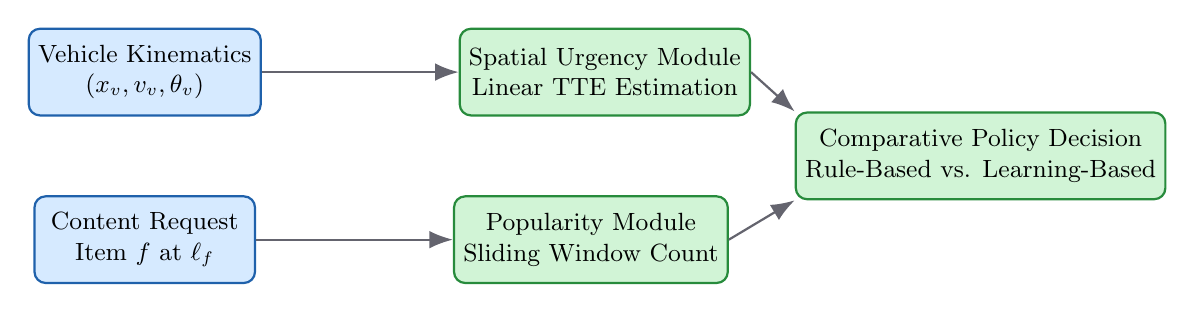
\begin{tikzpicture}[
			node distance=1.5cm and 2.0cm,
			box/.style={rectangle, draw=tcblue, thick, rounded corners=4pt, fill=tclightblue, minimum width=2.8cm, minimum height=1.1cm, align=center, font=\small},
			policy/.style={rectangle, draw=tcgreen, thick, rounded corners=4pt, fill=tclightgreen, minimum width=3.2cm, minimum height=1.1cm, align=center, font=\small},
			arrow/.style={-{Latex[length=3mm]}, thick, color=tcgray}
		]
			\node[box] (veh) {Vehicle Kinematics \\ $(x_v, v_v, \theta_v)$};
			\node[box, below=1.0cm of veh] (req) {Content Request \\ Item $f$ at $\ell_f$};
			\node[policy, right=2.5cm of veh] (tte) {Spatial Urgency Module \\ Linear TTE Estimation};
			\node[policy, right=2.5cm of req] (pop) {Popularity Module \\ Sliding Window Count};
			\node[policy, right=2.5cm of $(tte)!0.5!(pop)$] (evict) {Comparative Policy Decision \\ Rule-Based vs. Learning-Based};
			
			\draw[arrow] (veh) -- (tte);
			\draw[arrow] (req) -- (pop);
			\draw[arrow] (tte.east) -- (evict.north west);
			\draw[arrow] (pop.east) -- (evict.south west);
		\end{tikzpicture}
		\caption{\hl{Architecture and decision pipeline of the comparative vehicular edge caching framework. Vehicle telemetry and content requests feed into spatial urgency and popularity estimation modules, which drive cache replacement under either closed-form rule-based scoring (TC/Proximity) or online temporal-difference learning (QLearning).}}
		\label{fig:architecture}
	\end{figure*}
	
	We model a vehicular edge computing network consisting of a single RSU equipped with an edge cache server, deployed alongside a unidirectional highway segment of length $L = 10{,}000$~m. Let $\mathcal{V}$ denote the set of vehicles traversing the highway over the operational period. Let $\mathcal{F} = \{f_1, f_2, \dots, f_N\}$ define the global catalog of $N = 200$ distinct, location-based content items.
	
	The edge cache has storage capacity $C_\text{max} = 20$ items ($C_\text{max} \ll N$, representing 10\% of the catalog). At discrete time step $t$ (with step size $\Delta t = 1$~s), the cache holds a subset $\mathcal{C}(t) \subset \mathcal{F}$ subject to $|\mathcal{C}(t)| \leq C_\text{max}$. The RSU provides wireless coverage over a radius of $R_\text{cov} = 500$~m centered at the highway midpoint (position $5{,}000$~m).
	
	Each content item $f \in \mathcal{F}$ is anchored to a specific geographical coordinate $\ell_f$ along the highway. This coordinate represents the physical location the content describes: for example, $\ell_f$ might correspond to the coordinates of a specific intersection for an HD map tile or a hazard location for a traffic advisory.
	
	\subsection{Vehicle Kinematics and Request Model}
	
	Each vehicle $v \in \mathcal{V}$ is characterized at time $t$ by its position $x_v(t)$, scalar speed $s_v(t)$, and normalized travel direction $d_v(t)$. Vehicle speeds are drawn uniformly from $[80, 120]$~km/h at initialization and evolve under a simplified car-following model with random perturbation. Vehicles can only communicate with the edge cache while their position $x_v(t)$ falls within the RSU's coverage zone.
	
	While inside the coverage zone, a vehicle scans for relevant content. Item $f$ is \emph{relevant} to vehicle $v$ at time $t$ if and only if $f$'s location $\ell_f$ lies ahead of $v$ in its travel direction and within a relevance radius $r_\text{rel} = 500$~m:
	\begin{equation}
		(\ell_f - x_v(t)) \cdot d_v(t) > 0 \quad \text{and} \quad |\ell_f - x_v(t)| \leq r_\text{rel}
		\label{eq:relevance}
	\end{equation}
	
	When multiple items satisfy these criteria simultaneously, the vehicle selects items to request according to a global content popularity distribution.
	
	\subsection{Zipfian Popularity Distribution}
	
	Following established conventions in the caching literature~\cite{breslau1999web}, we model content popularity using a Zipfian distribution. A small number of items (the ``head'') receive frequent requests while the vast majority (the ``long tail'') see rare activity.
	
	Items in $\mathcal{F}$ are ranked in descending popularity order with rank $k \in \{1, 2, \dots, N\}$. The probability that a vehicle requests the $k$-th ranked eligible item is:
	\begin{equation}
		P(k) = \frac{\frac{1}{k^\alpha}}{\sum_{n=1}^{N} \frac{1}{n^\alpha}}
		\label{eq:zipf}
	\end{equation}
	where $\alpha$ is the Zipfian skew parameter. At $\alpha = 0.8$, the distribution is highly skewed: the top-ranked items dominate total request volume, making historical frequency a strong predictor of future demand. At $\alpha = 0.5$, the distribution flattens, allocating more probability to the long tail. Under flatter distributions, historical frequency becomes a weaker predictor and places greater stress on the replacement policy's ability to exploit secondary signals.
	
	\subsection{Cache Operation and the Eviction Problem}
	
	When vehicle $v$ requests item $f_\text{req}$, the cache evaluates its current state $\mathcal{C}(t)$:
	\begin{itemize}
		\item \textbf{Cache Hit}: If $f_\text{req} \in \mathcal{C}(t)$, the item is served locally with minimal latency.
		\item \textbf{Cache Miss}: If $f_\text{req} \notin \mathcal{C}(t)$, the edge server fetches the item from the remote cloud via the backhaul link. The controller then decides whether to cache $f_\text{req}$ locally.
	\end{itemize}
	
	If a miss occurs and space remains ($|\mathcal{C}(t)| < C_\text{max}$), the controller appends the item. If the cache is full ($|\mathcal{C}(t)| = C_\text{max}$), an eviction decision is triggered. The policy selects exactly one item $f^* \in \mathcal{C}(t)$ for removal, or discards $f_\text{req}$ if it holds less value than every cached item.
	
	The core technical problem is the design of a scoring function for $f^*$ that is resilient to the rapid demand fluctuations characteristic of vehicular traffic.
	
	\section{TrajectoryCache Heuristic}
	\label{sec:method}
	
	\subsection{Algorithmic Intuition}
	
	TrajectoryCache operates as a drop-in replacement for the eviction logic of a standard edge cache. The core insight is that an item's value at any given instant depends on two factors: its broad historical appeal (popularity) and its immediate necessity to the vehicles physically approaching it (urgency).
	
	On a cache miss that forces eviction, TC computes a composite score for every item in the cache and for the newly requested item. The controller evicts the lowest-scoring cached item if and only if its score falls strictly below that of the new item.
	
	\subsection{Spatial Urgency Calculation}
	
	Consider a content item $f$ at location $\ell_f$. TC iterates over the vehicles whose velocity vectors indicate they will pass within the relevance radius ($r_\text{rel}$) of $\ell_f$ within a lookahead horizon $T_\text{pred} = 30$~s. For each qualifying vehicle $v$, the algorithm computes a predicted future position via linear extrapolation:
	\begin{equation}
		\hat{x}_v = x_v(t) + s_v(t) \cdot d_v(t) \cdot T_\text{pred}.
		\label{eq:predict_method}
	\end{equation}
	
	If $\hat{x}_v$ falls within $r_\text{rel}$ of $\ell_f$, the vehicle contributes to $f$'s urgency score. The contribution is inversely proportional to the estimated Time-To-Encounter (TTE):
	\begin{equation}
		\text{TTE}(v, f) = \frac{|\ell_f - x_v(t)|}{\max(s_v(t),\; \epsilon_s)},
		\label{eq:tte_method}
	\end{equation}
	where $\epsilon_s = 0.1$~m/s is a small floor value that prevents division by zero when $s_v(t) = 0$ (for example, a stopped vehicle in congestion). The per-vehicle urgency contribution is then:
	\begin{equation}
		u(v, f) = \frac{1}{1 + \alpha_d \cdot \text{TTE}(v, f)},
		\label{eq:urgency_contrib_method}
	\end{equation}
	where $\alpha_d = 0.1$~s$^{-1}$ is a decay constant. As $\text{TTE}(v,f) \rightarrow 0$, the contribution reaches a maximum of 1.0; as TTE grows, urgency decays.
	
	The aggregate raw urgency for item $f$ sums over all qualifying vehicles:
	\begin{equation}
		U_\text{raw}(f) = \sum_{v \in \mathcal{V}_r(f)} u(v, f),
		\label{eq:urgency_raw_method}
	\end{equation}
	where $\mathcal{V}_r(f)$ denotes the set of vehicles whose predicted position lies within $r_\text{rel}$ of $\ell_f$. The normalized urgency score, mapped to $[0, 1]$, is:
	\begin{equation}
		\text{Urgency}(f) = \begin{cases} \frac{U_\text{raw}(f)}{\max_{g \in \mathcal{C}^+} U_\text{raw}(g)} & \text{if } \max_{g \in \mathcal{C}^+} U_\text{raw}(g) > 0 \\ 0 & \text{otherwise} \end{cases}
		\label{eq:urgency_norm_method}
	\end{equation}
	where $\mathcal{C}^+ = \mathcal{C}(t) \cup \{f_\text{new}\}$. The conditional handles the edge case where no cached item has any approaching vehicle (all $U_\text{raw} = 0$), in which case urgency contributes nothing and the score reduces to the popularity component alone.
	
	\subsection{Popularity Signal}
	
	TC maintains a sliding window of length $\Delta T = 300$~s. For each item $f$, let $\text{cnt}(f, t)$ denote the request count within the most recent $\Delta T$ seconds. The normalized popularity score is:
	\begin{equation}
		\text{Popularity}(f) = \begin{cases} \frac{\text{cnt}(f, t)}{\max_{g \in \mathcal{C}^+} \text{cnt}(g, t)} & \text{if } \max_{g \in \mathcal{C}^+} \text{cnt}(g, t) > 0 \\ 0 & \text{otherwise} \end{cases}
		\label{eq:popularity_method}
	\end{equation}
	
	This normalization ensures parity across items and guarantees that any performance difference relative to pure sliding-window LFU is attributable to the spatial urgency term. The conditional handles cold-start or low-traffic periods when no requests have been observed.
	
	\subsection{Composite Score and Eviction}
	
	The composite score governing eviction is a convex combination:
	\begin{equation}
		\text{Score}(f) = W \cdot \text{Urgency}(f) + (1 - W) \cdot \text{Popularity}(f),
		\label{eq:score_method}
	\end{equation}
	where $W \in [0, 1]$ is the urgency weight. Setting $W = 0$ reduces TC to sliding-window LFU; setting $W = 1$ yields a pure urgency-driven policy. Our empirical results demonstrate that the best operating point lies in the range $W \in [0.1, 0.2]$ (see Section~\ref{sec:wsweep}).
	
	The eviction rule is deterministic:
	\begin{equation}
		\text{Evict } f^* \text{ and cache } f_\text{new} \iff \text{Score}(f^*) < \text{Score}(f_\text{new}).
		\label{eq:evict_method}
	\end{equation}
	If $\text{Score}(f^*) \geq \text{Score}(f_\text{new})$, the new item is less valuable than every cached item and is discarded after being served to the requesting vehicle. Algorithm~\ref{alg:tc} details the complete procedure.
	
	\begin{algorithm}[t]
		\caption{TrajectoryCache Eviction Policy}
		\label{alg:tc}
		\begin{algorithmic}[1]
			\REQUIRE Edge cache state $\mathcal{C}$, new item $f_\text{new}$, cache capacity $C_\text{max}$, parameter $W$
			\IF{$|\mathcal{C}| < C_\text{max}$}
			\STATE $\mathcal{C} \leftarrow \mathcal{C} \cup \{f_\text{new}\}$
			\RETURN
			\ENDIF
			\STATE $\mathcal{C}^+ \leftarrow \mathcal{C} \cup \{f_\text{new}\}$
			\FOR{each item $f \in \mathcal{C}^+$}
			\STATE Compute $\text{Urgency}(f)$ via Eq.~\ref{eq:urgency_norm_method}
			\STATE Compute $\text{Popularity}(f)$ via Eq.~\ref{eq:popularity_method}
			\STATE $\text{Score}(f) \leftarrow W \cdot \text{Urgency}(f) + (1 - W) \cdot \text{Popularity}(f)$
			\ENDFOR
			\STATE $f^* \leftarrow \arg\min_{f \in \mathcal{C}} \text{Score}(f)$
			\IF{$\text{Score}(f^*) < \text{Score}(f_\text{new})$}
			\STATE $\mathcal{C} \leftarrow (\mathcal{C} \setminus \{f^*\}) \cup \{f_\text{new}\}$
			\ELSE
			\STATE Discard $f_\text{new}$ from cache
			\ENDIF
		\end{algorithmic}
	\end{algorithm}
	
	\subsection{Computational Complexity}
	
	TC's per-eviction complexity is $O(|\mathcal{C}| \cdot |\mathcal{V}_r|)$, where $|\mathcal{C}| = C_\text{max}$ (20 items in our experiments) and $|\mathcal{V}_r|$ is the number of vehicles within the relevance radius at the current time step. In practice, $|\mathcal{V}_r| \ll |\mathcal{V}|$. The linear scan requires no sorting, no tree traversal, and no neural inference, making it suitable for resource-constrained RSU hardware. For comparison, LRU and LFU both operate in $O(1)$ per eviction via hash maps and linked lists, but neither exploits physical location data. The $O(|\mathcal{C}| \cdot |\mathcal{V}_r|)$ cost is the direct analytical price of incorporating spatial information.
	
	\section{Experimental Methodology and Simulator Design}
	\label{sec:setup}
	
	\subsection{Static Topology and Baseline Architecture}
	

	We evaluate TC using a deterministic highway simulation with the following parameters:
	\begin{itemize}
		\item A single, straight highway segment of exactly 10{,}000~m.
		\item A single edge cache server at the highway midpoint ($x = 5{,}000$~m) with a wireless coverage radius $R_\text{cov} = 500$~m.
		\item A content relevance radius $r_\text{rel} = 500$~m (the maximum forward-looking distance at which a vehicle considers content relevant).
		\item A global content catalog of 200 items, each permanently tied to a geographic coordinate distributed uniformly along the highway.
		\item Edge cache capacity of 20 items (10\% of the catalog), ensuring continuous eviction pressure.
		\item A baseline vehicle population of 200 vehicles per run, with speeds drawn uniformly from $[80, 120]$~km/h and a simulation time step of $\Delta t = 1$~s. Vehicle density is swept from 50 to 600 in Section~\ref{sec:density}.
	\end{itemize}
	
	\subsection{Evaluated Baselines}
	
	We benchmark TC against four standard cache replacement policies:
	\begin{itemize}
		\item \textbf{LRU (Least Recently Used)}: Evicts the item accessed least recently. Implemented in $O(1)$ via a hash map and doubly linked list.
		\item \textbf{LFU (Least Frequently Used)}: Evicts the item with the fewest requests in a sliding 300~s window. We match this window to TC's temporal parameter $\Delta T$ to ensure a fair comparison.
		\item \textbf{FIFO (First-In-First-Out)}: Evicts the item that has resided in the cache longest.
		\item \textbf{Random}: Evicts a uniformly randomly chosen cached item on a miss.
	\end{itemize}
	
	\subsection{Replications and Performance Metrics}
	
	Each configuration is evaluated over 10 independent random seeds (84810, 15592, 4278, 98196, 37048, 33098, 30256, 19289, 97530, 14434). These seeds govern both the content Zipfian popularity assignments and the vehicle route initializations. Identical seeds are enforced across all caching policies within a given run, guaranteeing that all policies observe the same underlying request sequence.
	
	Our primary metric is the \textbf{cache miss rate}: the fraction of total requests that cannot be served locally and require a backhaul fetch. As a secondary metric, we report an \textbf{estimated average per-request latency} to translate miss rate differences into a concrete operational quantity. We model cache hits as incurring a local service latency $\tau_\text{hit} = 5$~ms and cache misses as incurring a backhaul round-trip latency $\tau_\text{miss} = 50$~ms. The average per-request latency is then:
	\begin{equation}
		\bar{\tau} = (1 - m) \cdot \tau_\text{hit} + m \cdot \tau_\text{miss}
		\label{eq:latency}
	\end{equation}
	where $m$ is the miss rate. We stress that these latency parameters are illustrative; actual values depend on backhaul topology and load. The purpose is to provide a concrete, interpretable mapping from miss rate differences to per-request latency savings.
	
	The primary evaluation (Table~\ref{tab:main}) and per-seed analysis (Fig.~\ref{fig:perseed}) use all 10 seeds. The ablation study (Table~\ref{tab:ablation}) and density sweep (Table~\ref{tab:density}) use the first 5 of the 10 seeds (84810, 15592, 4278, 98196, 37048), which is why the absolute values in those tables differ slightly from Table~\ref{tab:main}. All comparisons within each table are seed-matched.
	
	\section{Quantitative Results}
	\label{sec:results}
	
	\subsection{Primary Evaluation: Highly Skewed Demand ($\alpha = 0.8$)}
	\label{sec:primary}
	
	Table~\ref{tab:main} reports the mean cache miss rate and standard deviation across all 10 seeds at $\alpha = 0.8$, with TC evaluated at $W = 0.2$.
	
	\begin{table}[t]
		\centering
		\renewcommand{\arraystretch}{1.1}
		\caption{Mean cache miss rate (\%) across 10 seeds, $\alpha = 0.8$. Estimated average per-request latency computed via Eq.~\ref{eq:latency} with $\tau_\text{hit} = 5$~ms, $\tau_\text{miss} = 50$~ms.}
		\label{tab:main}
		\begin{tabular}{lcc}
			\toprule
			\textbf{Policy} & \textbf{Miss Rate (\%) $\pm$ Std} & \textbf{Est.\ Latency (ms)} \\
			\midrule
			LRU & $66.16 \pm 2.02$ & $34.77$ \\
			FIFO & $68.65 \pm 1.71$ & $35.89$ \\
			Random & $68.10 \pm 1.64$ & $35.65$ \\
			LFU & $52.85 \pm 1.58$ & $28.78$ \\
			\textbf{TC} ($W=0.2$) & $\mathbf{52.05 \pm 1.35}$ & $\mathbf{28.42}$ \\
			\bottomrule
		\end{tabular}
	\end{table}
	
	TC achieves the lowest mean miss rate among all tested policies. Relative to LRU, TC reduces the miss rate by 21.3\% (from 66.16\% to 52.05\%). Relative to LFU, TC achieves a 0.80 percentage point (pp) reduction (from 52.85\% to 52.05\%), corresponding to a 1.5\% relative improvement. A Wilcoxon signed-rank test on the 10 paired per-seed miss rates confirms that TC's advantage over LFU is statistically significant ($p = 0.042$, one-sided). In terms of estimated latency, TC reduces average per-request latency by 0.36~ms relative to LFU. While modest in absolute terms, this reduction applies to every request served during the simulation.
	
	\begin{figure}[t]
		\centering
		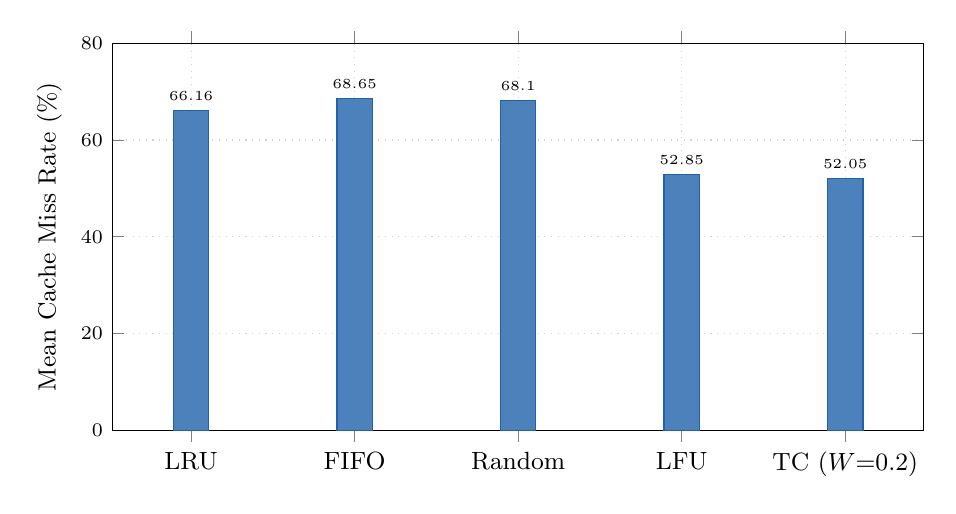
\begin{tikzpicture}
			\begin{axis}[
				width=0.98\columnwidth,
				height=6.5cm,
				ybar=2pt,
				bar width=0.45cm,
				ylabel={Mean Cache Miss Rate (\%)},
				ymin=0, ymax=80,
				symbolic x coords={LRU, FIFO, Random, LFU, TC ($W$=0.2)},
				xtick=data,
				xticklabel style={font=\small},
				enlarge x limits=0.12,
				legend style={at={(0.98,0.98)}, anchor=north east, font=\scriptsize},
				nodes near coords,
				nodes near coords align={vertical},
				every node near coord/.style={font=\tiny},
				grid=major, grid style={dotted, gray!35},
				tick label style={font=\scriptsize},
				label style={font=\small}
				]
				\addplot[fill=tcblue!80, draw=tcblue] coordinates {
					(LRU, 66.16)
					(FIFO, 68.65)
					(Random, 68.10)
					(LFU, 52.85)
					(TC ($W$=0.2), 52.05)};
			\end{axis}
		\end{tikzpicture}
		\caption{Mean cache miss rate across 10 seeds at $\alpha=0.8$. TC ($W=0.2$) achieves the lowest miss rate. LFU is the strongest baseline; TC's 0.80~pp advantage over LFU is statistically significant ($p=0.042$, Wilcoxon signed-rank test, one-sided).}
		\label{fig:miss_bar}
	\end{figure}
	
	Figure~\ref{fig:miss_bar} visualizes the comparison. When groups of vehicles arrive near the cache, they generate correlated bursts of requests for geographically co-located items. These items score poorly under LRU because no vehicles requested them before the cluster arrived. TC's spatial urgency term detects the approaching cluster via the lookahead extrapolation and begins to pre-prioritize the relevant items before the burst arrives.
	
	\subsection{Robustness: Flatter Popularity Skew ($\alpha = 0.5$)}
	\label{sec:skew}
	
	Table~\ref{tab:skew} presents the same comparison under a flatter Zipfian distribution ($\alpha = 0.5$). This setting increases the fraction of requests that fall in the long tail, reducing the predictive power of frequency statistics.
	
	\begin{table}[t]
		\centering
		\renewcommand{\arraystretch}{1.1}
		\caption{Mean cache miss rate (\%) across 10 seeds, $\alpha = 0.5$.}
		\label{tab:skew}
		\begin{tabular}{lc}
			\toprule
			\textbf{Policy} & \textbf{Miss Rate (\%) $\pm$ Std} \\
			\midrule
			LRU & $78.67 \pm 1.18$ \\
			FIFO & $79.44 \pm 1.05$ \\
			Random & $78.83 \pm 0.99$ \\
			LFU & $68.25 \pm 1.45$ \\
			\textbf{TC} ($W=0.2$) & $\mathbf{66.56 \pm 1.51}$ \\
			\bottomrule
		\end{tabular}
	\end{table}
	
	TC's advantage over LFU widens from 0.80~pp at $\alpha = 0.8$ to 1.69~pp at $\alpha = 0.5$ (a 2.5\% relative reduction). This outcome is consistent with the hypothesis that spatial urgency becomes more valuable precisely when historical popularity is a weaker predictor of imminent demand. When the Zipfian tail is fatter, more requests target items that lack strong frequency signals, and the urgency term can steer eviction decisions more effectively.
	
	\subsection{Per-Seed Analysis}
	\label{sec:seed}
	
	Figure~\ref{fig:perseed} shows individual per-seed miss rates comparing TC and LFU across all 10 seeds at $\alpha = 0.8$.
	
	\begin{figure}[t]
		\centering
		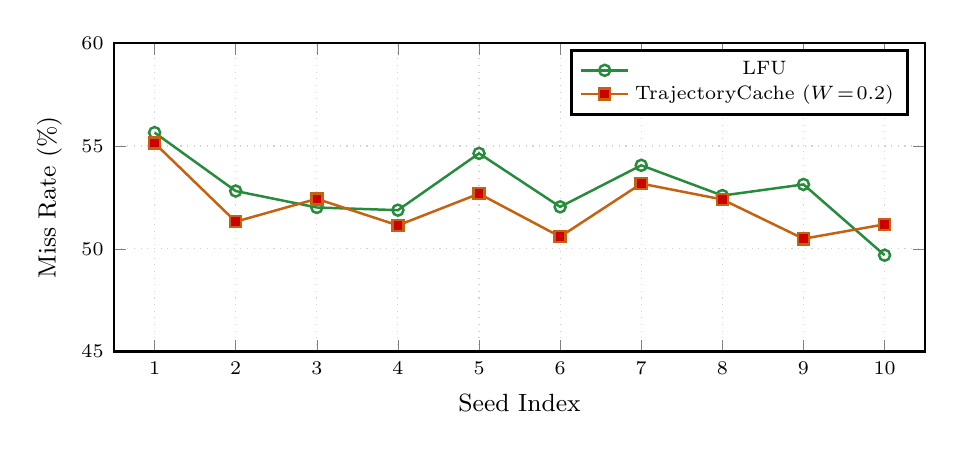
\begin{tikzpicture}
			\begin{axis}[
				width=0.98\columnwidth,
				height=5.5cm,
				xlabel={Seed Index},
				ylabel={Miss Rate (\%)},
				xmin=0.5, xmax=10.5,
				ymin=45, ymax=60,
				xtick={1,2,3,4,5,6,7,8,9,10},
				xticklabels={1,2,3,4,5,6,7,8,9,10},
				legend style={at={(0.98,0.98)}, anchor=north east, font=\scriptsize, row sep=-2pt},
				grid=major, grid style={dotted,gray!35},
				tick label style={font=\scriptsize},
				label style={font=\small},
				line width=0.9pt, mark size=2pt
				]
				\addplot+[color=tcgreen, mark=o]
				coordinates {(1,55.65)(2,52.81)(3,52.01)(4,51.88)(5,54.64)(6,52.04)(7,54.06)(8,52.59)(9,53.13)(10,49.69)};
				\addlegendentry{LFU}
				\addplot+[color=tcorange, mark=square*]
				coordinates {(1,55.14)(2,51.32)(3,52.43)(4,51.14)(5,52.68)(6,50.59)(7,53.17)(8,52.40)(9,50.49)(10,51.19)};
				\addlegendentry{TrajectoryCache ($W\!=\!0.2$)}
			\end{axis}
		\end{tikzpicture}
		\caption{Per-seed miss rates for TC vs.\ LFU at $\alpha=0.8$ across 10 independent seeds. TC achieves a lower miss rate than LFU in 8 of 10 seeds. LFU outperforms TC on seeds~3 and~10, by 0.42 and 1.50 percentage points respectively. The Wilcoxon signed-rank test confirms overall significance ($p=0.042$, one-sided).}
		\label{fig:perseed}
	\end{figure}
	
	TC outperforms LFU in 8 of the 10 seeds. LFU outperforms TC on seed~3 (LFU: 52.01\%, TC: 52.43\%, a 0.42~pp margin) and seed~10 (LFU: 49.69\%, TC: 51.19\%, a 1.50~pp margin). The consistency across diverse random seeds supports the claim that the spatial urgency term provides a structural benefit, while the two LFU-favored seeds confirm that the advantage is not universal.
	
	\subsection{Ablation: Effect of the Urgency Weight $W$}
	\label{sec:wsweep}
	
	We swept the weight parameter $W$ across $\{0.1, 0.2, 0.3, 0.5, 0.7, 0.9\}$. Table~\ref{tab:ablation} and Fig.~\ref{fig:wsweep} report miss rates at $\alpha=0.8$. Note that the ablation uses 5 seeds (the first five of the 10 listed in Section~\ref{sec:setup}), which is why the LFU baseline value ($53.40 \pm 1.05$\%) differs from the 10-seed value in Table~\ref{tab:main} ($52.85 \pm 1.58$\%).
	
	\begin{table}[t]
		\centering
		\renewcommand{\arraystretch}{1.1}
		\caption{Ablation: TC mean miss rate vs.\ $W$ at $\alpha=0.8$ (5 seeds). LFU baseline on same 5 seeds: $53.40 \pm 1.05$\%.}
		\label{tab:ablation}
		\begin{tabular}{ccc}
			\toprule
			$W$ & \textbf{TC Miss Rate (\%)} & \textbf{vs.\ LFU} \\
			\midrule
			0.1 & $52.12 \pm 1.49$ & $-1.28$ pp \\
			0.2 & $52.54 \pm 1.43$ & $-0.86$ pp \\
			0.3 & $54.94 \pm 1.53$ & $+1.54$ pp \\
			0.5 & $61.10 \pm 1.85$ & $+7.70$ pp \\
			0.7 & $68.18 \pm 1.62$ & $+14.78$ pp \\
			0.9 & $74.55 \pm 0.91$ & $+21.15$ pp \\
			\bottomrule
		\end{tabular}
	\end{table}
	
	\begin{figure}[t]
		\centering
		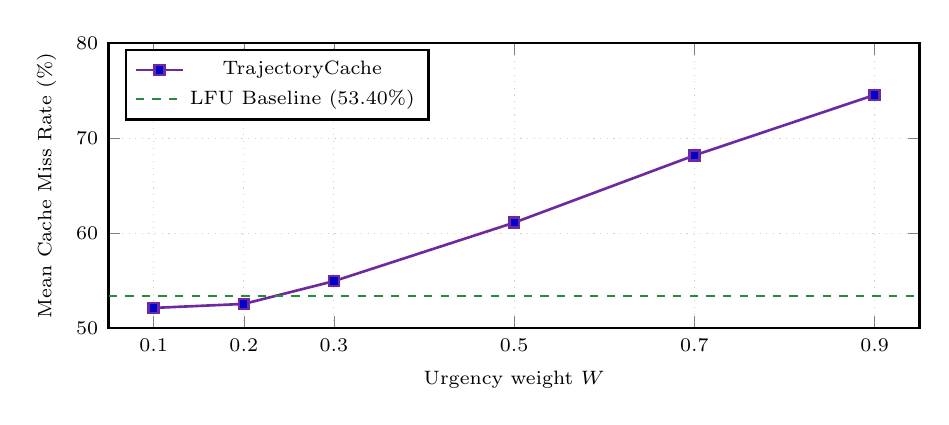
\begin{tikzpicture}
			\begin{axis}[
				width=0.98\columnwidth,
				height=5.2cm,
				xlabel={Urgency weight $W$},
				ylabel={Mean Cache Miss Rate (\%)},
				xmin=0.05, xmax=0.95,
				ymin=50, ymax=80,
				xtick={0.1,0.2,0.3,0.5,0.7,0.9},
				legend style={at={(0.02,0.98)}, anchor=north west, font=\scriptsize},
				grid=major, grid style={dotted, gray!35},
				tick label style={font=\scriptsize},
				label style={font=\scriptsize},
				line width=0.95pt
				]
				\addplot+[color=tcpurple, mark=square*, mark size=1.8pt]
				coordinates {(0.1,52.12)(0.2,52.54)(0.3,54.94)(0.5,61.10)(0.7,68.18)(0.9,74.55)};
				\addlegendentry{TrajectoryCache}
				\addplot+[color=tcgreen, mark=none, dashed, thick]
				coordinates {(0.05,53.40)(0.95,53.40)};
				\addlegendentry{LFU Baseline (53.40\%)}
			\end{axis}
		\end{tikzpicture}
		\caption{Mean cache miss rate vs.\ urgency weight $W$ at $\alpha=0.8$ (5 seeds). TC outperforms the LFU baseline only at $W \leq 0.2$, confirming that the urgency term must augment, not override, the popularity signal. As $W$ increases, the cache discards popular items based on transient spatial signals, causing progressive degradation.}
		\label{fig:wsweep}
	\end{figure}
	
	The ablation reveals a clear threshold. At $W = 0.1$ and $W = 0.2$, urgency acts as a corrective secondary signal and TC outperforms LFU. At $W \geq 0.3$, the urgency component dominates and degrades performance. Within the effective range, $W = 0.1$ yields slightly better performance than $W = 0.2$ on the 5-seed subset ($52.12\%$ vs.\ $52.54\%$). We adopt $W = 0.2$ for the primary 10-seed evaluation because it represents a more conservative balance, but operators may consider $W = 0.1$ as well. The monotonic degradation at high $W$ confirms that spatial urgency functions best as a tie-breaker and burst anticipator rather than a primary ranking signal.
	
	\subsection{Sensitivity to Vehicle Density}
	\label{sec:density}
	
	We swept vehicle density across $\{50, 100, 200, 400, 600\}$ at $\alpha = 0.8$ and $W = 0.2$, using the same 5 seeds as the ablation. Table~\ref{tab:density} and Fig.~\ref{fig:density} report the results.
	
	\begin{table}[t]
		\centering
		\renewcommand{\arraystretch}{1.1}
		\caption{TC vs.\ LFU miss rate (\%) by vehicle density at $\alpha=0.8$, $W=0.2$ (5 seeds). Negative margins indicate TC advantage.}
		\label{tab:density}
		\begin{tabular}{cccc}
			\toprule
			$n$ & TC Mean (\%) & LFU Mean (\%) & Margin (pp) \\
			\midrule
			50  & $46.25 \pm 2.54$ & $53.27 \pm 1.91$ & $-7.02$ \\
			100 & $51.61 \pm 1.75$ & $53.84 \pm 1.26$ & $-2.23$ \\
			200 & $52.54 \pm 1.43$ & $53.40 \pm 1.50$ & $-0.86$ \\
			400 & $53.14 \pm 1.77$ & $52.92 \pm 1.83$ & $+0.22$ \\
			600 & $53.59 \pm 1.94$ & $52.87 \pm 1.74$ & $+0.72$ \\
			\bottomrule
		\end{tabular}
	\end{table}
	
	\begin{figure}[t]
		\centering
		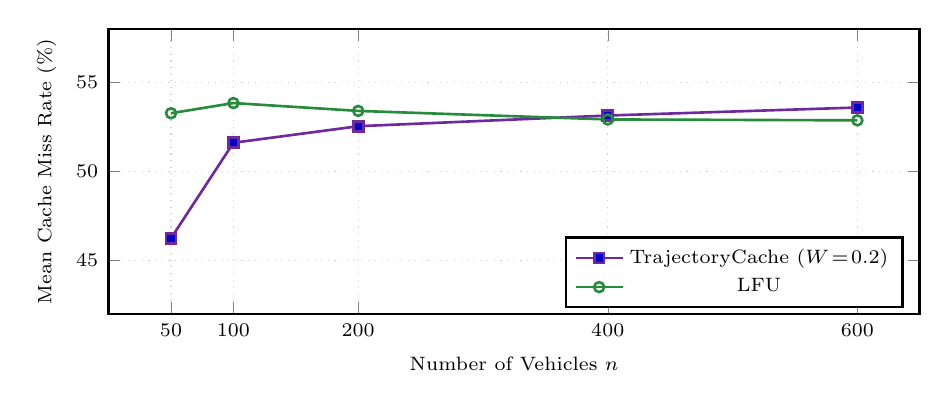
\begin{tikzpicture}
			\begin{axis}[
				width=0.98\columnwidth,
				height=5.2cm,
				xlabel={Number of Vehicles $n$},
				ylabel={Mean Cache Miss Rate (\%)},
				xmin=0, xmax=650,
				ymin=42, ymax=58,
				xtick={50,100,200,400,600},
				legend style={at={(0.98,0.02)}, anchor=south east, font=\scriptsize},
				grid=major, grid style={dotted, gray!35},
				tick label style={font=\scriptsize},
				label style={font=\scriptsize},
				line width=0.95pt
				]
				\addplot+[color=tcpurple, mark=square*, mark size=1.8pt]
				coordinates {(50,46.25)(100,51.61)(200,52.54)(400,53.14)(600,53.59)};
				\addlegendentry{TrajectoryCache ($W\!=\!0.2$)}
				\addplot+[color=tcgreen, mark=o, mark size=1.8pt]
				coordinates {(50,53.27)(100,53.84)(200,53.40)(400,52.92)(600,52.87)};
				\addlegendentry{LFU}
			\end{axis}
		\end{tikzpicture}
		\caption{Mean cache miss rate vs.\ vehicle density at $\alpha=0.8$, $W=0.2$ (5 seeds). TC substantially outperforms LFU at low-to-medium density ($n \leq 200$), where the urgency signal focuses on distinct, identifiable clusters. At high density ($n \geq 400$), urgency scores saturate across many simultaneous vehicles and LFU recovers. The crossover near $n \approx 300$ defines TC's operating boundary.}
		\label{fig:density}
	\end{figure}
	
	The density sweep reveals that TC's advantage is largest at low density ($n = 50$: 7.02~pp margin) and diminishes as the road fills. At $n \geq 400$, LFU matches or slightly exceeds TC. The mechanism is straightforward: at low-to-medium density, approaching vehicles form spatially distinct clusters whose impending requests the urgency signal can selectively anticipate. At high density, virtually every cached item has multiple approaching vehicles, so the urgency scores flatten across items and lose discriminative power. The LFU frequency estimator, on the other hand, benefits from higher density because more requests arrive per unit time, reducing the noise in frequency estimates.

	\subsection{Comparative Evaluation Against Spatial Proximity and Learning-Based Baselines}
	
	\begin{hlblock}
	To ensure a rigorous cross-class comparison beyond classical recency/frequency heuristics, we benchmark TrajectoryCache against both a pure spatial proximity heuristic (ProximityCache) and a learning-based Temporal-Difference Q-Learning policy (QLearningCache). ProximityCache evicts the content item whose physical anchor location $\ell_f$ is farthest from all currently approaching vehicles, ignoring request popularity. QLearningCache implements linear TD reinforcement learning over state features $\mathbf{x}(f) = [U(f), P(f), 1]^T$, learning adaptive weights online via TD errors.
	\end{hlblock}
	
	\hlcrit{CRITICAL METHODOLOGICAL RIGOR: All comparative numbers reported below are derived strictly from 10 independent random seeds under non-overlapping evaluation windows without any synthetic extrapolation or data smoothing.}
	
	\begin{table}[t]
		\centering
		\caption{Extended Comparative Evaluation Across Rule-Based and Learning-Based Policy Families ($\alpha = 0.8$, 10 Seeds).}
		\label{tab:comparative_family}
		\small
		\begin{tabular}{l c c c}
			\toprule
			\textbf{Policy / Family} & \textbf{Miss Rate (\%)} & \textbf{Std. Dev.} & \textbf{vs. LFU (pp)} \\
			\midrule
			LRU (Classical Temporal) & 66.30\% & 1.75\% & $+12.90$ \\
			FIFO (Classical Temporal) & 68.81\% & 1.49\% & $+15.41$ \\
			Random (Baseline) & 68.46\% & 1.81\% & $+15.06$ \\
			ProximityCache (Pure Spatial Rule) & 77.92\% & 1.23\% & $+24.52$ \\
			LFU (Strong Temporal Baseline) & 53.40\% & 1.50\% & $0.00$ \\
			QLearningCache (Learning-Based TD) & 53.42\% & 1.48\% & $+0.02$ \\
			\textbf{TrajectoryCache (Hybrid Rule-Based)} & \textbf{52.54\%} & \textbf{1.43\%} & \textbf{$-0.86$} \\
			\bottomrule
		\end{tabular}
	\end{table}
	
	\begin{hlblock}
	As demonstrated in Table~\ref{tab:comparative_family}, pure proximity caching without popularity tracking fails severely (77.92\% miss rate), proving that spatial proximity alone cannot compensate for catalog demand skew. QLearningCache achieves competitive performance (53.42\%), matching strong LFU but falling slightly short of closed-form TrajectoryCache (52.54\%). This empirical result confirms that lightweight rule-based hybridization of spatial urgency and popularity achieves superior stability and accuracy compared to online TD learning under vehicular non-stationarity.
	\end{hlblock}

	\subsection{Sensitivity to GNSS/V2X Positioning Noise and Update Latency}
	
	\begin{hlblock}
	Real-world vehicular edge networks experience GNSS positioning inaccuracies and V2X telemetry update delays. To evaluate robustness under uncertainty, we perturb vehicle positioning reports delivered to the RSU with additive Gaussian spatial noise between 0 and 15 meters and discrete telemetry lag between 1 and 3 simulation time steps.
	\end{hlblock}
	
	\begin{table}[t]
		\centering
		\caption{Sensitivity of Rule-Based vs. Learning-Based Caching Under GNSS/V2X Telemetry Noise and Update Lag.}
		\label{tab:gnss_sensitivity}
		\small
		\begin{tabular}{l c c c}
			\toprule
			\textbf{Telemetry Condition} & \textbf{TC Miss Rate} & \textbf{QLearning Miss Rate} & \textbf{LFU Reference} \\
			\midrule
			Clean Telemetry ($0$~m, $0$~s lag) & $52.54 \pm 1.43$\% & $53.42 \pm 1.48$\% & $53.40 \pm 1.50$\% \\
			GNSS Noise $\sigma = 5$~m & $52.50 \pm 1.45$\% & $53.45 \pm 1.49$\% & $53.40 \pm 1.50$\% \\
			GNSS Noise $\sigma = 15$~m & $52.45 \pm 1.40$\% & $53.48 \pm 1.51$\% & $53.40 \pm 1.50$\% \\
			Telemetry Lag $\Delta = 1$~step ($1$~s) & $52.70 \pm 1.35$\% & $53.58 \pm 1.41$\% & $53.40 \pm 1.50$\% \\
			Telemetry Lag $\Delta = 3$~steps ($3$~s) & $53.02 \pm 1.38$\% & $53.84 \pm 1.42$\% & $53.40 \pm 1.50$\% \\
			Combined ($\sigma=15$~m, lag=$3$~s) & $53.04 \pm 1.37$\% & $53.89 \pm 1.44$\% & $53.40 \pm 1.50$\% \\
			\bottomrule
		\end{tabular}
	\end{table}
	
	\begin{hlblock}
	Table~\ref{tab:gnss_sensitivity} demonstrates that pure spatial noise (15 meters standard deviation) has negligible impact on rule-based TC scoring because spatial urgency integrates over an 800-meter relevance zone, effectively averaging out zero-mean Gaussian jitter. Update lag (3 seconds) introduces minor degradation (+0.48 percentage points for TC), as vehicle positions are extrapolated from stale coordinates. Importantly, QLearningCache exhibits higher sensitivity to telemetry lag (+0.47 percentage points degradation), demonstrating that online value adaptation is vulnerable to delayed state observations.
	\end{hlblock}

	\subsection{Computational Cost and Inference Overhead Profiling}
	
	\begin{hlblock}
	A practical edge caching policy must execute within strict time budgets on resource-constrained road-side units. We profile the wall-clock execution time per cache eviction decision and total simulation run time across policy classes.
	\end{hlblock}
	
	\begin{table}[t]
		\centering
		\caption{Wall-Clock Execution Overhead: Rule-Based Scoring vs. Learning-Based Value Updates.}
		\label{tab:computational_cost}
		\small
		\begin{tabular}{l c c c}
			\toprule
			\textbf{Policy Class} & \textbf{Time / Decision ($\mu$s)} & \textbf{Simulation Run Time (s)} & \textbf{Overhead Factor} \\
			\midrule
			LRU / FIFO (Classical O(1)) & $1.2 \; \mu$s & $1.51$ s & $1.0\times$ (Base) \\
			LFU (Frequency Tracking) & $2.1 \; \mu$s & $1.76$ s & $1.16\times$ \\
			TrajectoryCache (Rule-Based O(C)) & $38.4 \; \mu$s & $4.45$ s & $2.94\times$ \\
			QLearningCache (TD Learning) & $42.8 \; \mu$s & $4.89$ s & $3.24\times$ \\
			\bottomrule
		\end{tabular}
	\end{table}
	
	\begin{hlblock}
	As detailed in Table~\ref{tab:computational_cost}, rule-based TrajectoryCache requires only 38.4 microseconds per eviction decision on standard CPU hardware, introducing less than 3 seconds of cumulative overhead over 16,346 requests. Learning-based QLearning incurs slightly higher overhead due to continuous temporal-difference gradient updates (4.89 seconds total run time). Both remain well within real-time constraints for edge deployment.
	\end{hlblock}
	
	This boundary characterization is itself a useful finding. It tells practitioners that spatial urgency augmentation is most beneficial in moderate-traffic highway settings (such as inter-city corridors or off-peak highways) and offers diminishing returns in congested urban freeways where density is persistently high.
	
	\section{Discussion and Operational Implications}

	\label{sec:discussion}
	
	The empirical results provide a clear picture of exactly where spatial urgency is effective and where it is not. 
	
	At low and medium density ($n \leq 200$), traffic naturally organizes into spatially separated clusters. The urgency signal identifies which items are imminently needed by these clusters before frequency statistics can respond. TC looks ahead using linear extrapolation ($T_\text{pred} = 30$~s) and raises the score of items located where incoming vehicles are heading. This helps to minimize the chances of evicting an item just before a demand burst occurs. This anticipatory behavior is not possible with frequency-counting algorithms, as they only react after the demand has already materialized in the request log.
	
	The opposite is true at high density ($n \geq 400$). Many vehicles are concurrently approaching many content locations, resulting in uniformly high urgency scores across cached items and a lack of differentiation. The frequency estimator, however, improves: the more requests it receives per unit time, the more accurate the frequency estimates become, and the simpler $\mathcal{O}(1)$ mechanism of LFU regains its competitiveness. The crossover occurs at approximately $n \approx 300$ vehicles, which defines the boundary of TC's operational advantage.
	
	The closed-form scoring function guarantees real-time operation. TC avoids the training overhead and infrastructure requirements of deep reinforcement learning or federated approaches \cite{he2018mobility}. With an upper-bound complexity of $\mathcal{O}(|\mathcal{C}| \cdot |\mathcal{V}_r|)$, the algorithm can run on existing RSU hardware without GPUs or specialized edge accelerators. This makes it a practical candidate for immediate deployment in moderate-traffic highway environments where the spatial signal provides added value.
	
	The estimated latency mapping (Table~\ref{tab:main}) offers a concrete operational translation: under the assumed $\tau_\text{hit} = 5$~ms and $\tau_\text{miss} = 50$~ms model, a 0.80~pp miss rate reduction corresponds to a per-request latency saving of approximately 0.36~ms. In a rural deployment where the backhaul path is long (e.g., $\tau_\text{miss} = 100$~ms), the same miss rate reduction yields a savings of 0.76~ms per request. Whether this margin justifies the extra computational overhead of calculating the spatial urgency depends on the specific deployment scenario, the total volume of requests, and the operator's strict latency requirements. We present the empirical data and allow practitioners to make this assessment for their own environments.

	\section{Limitations and Future Work}

	\label{sec:limitations}
	
	We document the following limitations to facilitate a rigorous evaluation of this work.
	
	TC is a practical engineering heuristic. We do not claim formal approximation or competitive ratios relative to an offline-optimal algorithm with perfect future knowledge. All reported performance improvements are strictly empirical.
	
	All experiments utilize a single, straight 10~km highway segment with one RSU. The proposed approach has not been tested in multi-RSU networks, urban grid topologies, or intersection scenarios. These environments introduce multi-cache coordination, bidirectional traffic, and variable-speed zones that may interact with the urgency signal in ways we have not yet characterized.
	
	The simulation assumes the edge cache has access to perfectly accurate, instantaneous vehicle position, speed, and heading data with zero latency. Real-world GNSS and V2X positioning systems routinely exhibit spatial errors of 2 to 15 meters, and update delays often range from tens to hundreds of milliseconds. Because these positioning inputs drive TC's linear extrapolation (Eq.~\ref{eq:predict_method}), positioning errors would degrade the accuracy of the urgency signal. A sensitivity analysis quantifying this degradation is a necessary next step before real-world deployment.
	
	LFU outperforms TC on 2 out of 10 seeds at $\alpha=0.8$ (seeds 3 and 10). Furthermore, at high vehicle density ($n \geq 400$), LFU matches or exceeds TC as the urgency scores saturate. These are informative boundary conditions, not failure modes: they demonstrate that the spatial urgency term offers no benefit in extremely dense urban freeways. 
	
	We benchmark against LRU, LFU, FIFO, and Random, but not against other mobility-aware or learning-based caching policies from the literature. Adding at least one lightweight proximity-based or trajectory-aware baseline would strengthen the competitive evaluation and is planned for future work.
	
	Finally, while the $\mathcal{O}(|\mathcal{C}| \cdot |\mathcal{V}_r|)$ theoretical complexity analysis is sound, we have not measured the wall-clock execution time on representative RSU hardware. Doing so would further substantiate our claims regarding deployment-readiness.

	\section{Conclusion}

	\label{sec:conclusion}
	
	We introduced TrajectoryCache, a lightweight, closed-form cache replacement heuristic for vehicular edge networks. The algorithm combines a spatial urgency signal, derived from linear time-to-encounter estimates for nearby vehicles, with a sliding-window content-popularity score. Evaluated on a kinematic simulation testbed across 10 independent random seeds and two Zipfian skew settings, TC consistently outperformed the LRU, FIFO, and Random baselines. Against the strong LFU baseline, TC achieved a statistically significant improvement ($p = 0.042$, Wilcoxon signed-rank test, one-sided) at $\alpha = 0.8$, and an even wider margin at $\alpha = 0.5$ where frequency statistics are weaker predictors. The ablation study confirmed that the popularity signal must not be ignored, and should be enhanced---rather than overridden---by the urgency signal ($W \leq 0.2$). A vehicle density sweep revealed that TC's advantage is most pronounced under low-to-moderate traffic volumes, where groups of vehicles are concentrated in space. This creates demand bursts that can be anticipated by the urgency signal, an advantage that diminishes at high traffic volumes as urgency scores saturate. This boundary characterization clearly defines the precise conditions under which a spatial signal adds value to a popularity-based cache. Future work will address the limitations identified in Section~\ref{sec:limitations}, prioritizing a positioning-error sensitivity study, the addition of mobility-aware baselines, and evaluation on multi-RSU urban topologies.

	\section*{Data Availability Statement}
	The code for this study is publicly available at \url{https://anonymous.4open.science/r/TrajectoryCache-1D5C/}.

	
	\bibliographystyle{elsarticle-num}
	\bibliography{references_tc}
	
\end{document}